\documentclass[french, a4paper, 12pt, openany]{report}
% General packages
\usepackage{amsfonts, amssymb, amsthm}
\usepackage{array}
\usepackage{enumitem}
\usepackage{mathtools}
\usepackage{stmaryrd}
\usepackage{empheq, environ} % packages for system environment
\usepackage{calrsfs} % better mathcal letters
\usepackage{graphicx}


% Layout
\usepackage{fancyhdr, fancyvrb}
\usepackage{lastpage}
\usepackage[left=2.0cm, right=2.0cm, top = 2.0cm, bottom = 2.0cm]{geometry}
\usepackage{lettrine, yfonts}
\usepackage{multicol}
\usepackage{minitoc}
\usepackage{hyperref}
\hypersetup{hyperindex=true, colorlinks, linkcolor=blue, urlcolor=blue, citecolor=blue, breaklinks=true}
\everymath{\displaystyle}


% Language
\usepackage[utf8]{inputenc}
\usepackage[T1]{fontenc}
\usepackage{babel}


% Minted
\newcommand{\python}{\mintinline[breaklines=true, breakanywhere=true]{python}}
\newminted{python}{
	linenos=true,
	tabsize=4,
	breaklines=true,
	fontfamily=courier,
	autogobble,
	style=rainbow_dash,
	xleftmargin=5pt,
	xrightmargin=5pt,
	frame=lines
}


% Pagestyle
\everymath{\displaystyle}
\pagestyle{fancy}
\fancypagestyle{plain}


% Customs commands and environnements
\renewcommand{\leq}{\leqslant}
\renewcommand{\geq}{\geqslant}
\renewcommand{\ker}{\mathrm{Ker\,}}
\renewcommand{\vec}{\overrightarrow}
\newcommand{\im}{\mathrm{Im\,}}
\newcommand{\derivative}[2]{\frac{\mathrm{d} #1}{\mathrm{d}#2}}
\newcommand{\enluminure}[2]{\lettrine[lines=3]{\small \initfamily #1}{#2}}
\newcommand{\nnchapter}[1]{
	\chapter*{#1}
	\addstarredchapter{#1}
	\markboth{\uppercase{#1}}{}		
}

\def\restriction#1#2{\mathchoice
              {\setbox1\hbox{${\displaystyle #1}_{\scriptstyle #2}$}
              \restrictionaux{#1}{#2}}
              {\setbox1\hbox{${\textstyle #1}_{\scriptstyle #2}$}
              \restrictionaux{#1}{#2}}
              {\setbox1\hbox{${\scriptstyle #1}_{\scriptscriptstyle #2}$}
              \restrictionaux{#1}{#2}}
              {\setbox1\hbox{${\scriptscriptstyle #1}_{\scriptscriptstyle #2}$}
              \restrictionaux{#1}{#2}}}
\def\restrictionaux#1#2{{#1\,\smash{\vrule height .8\ht1 depth .85\dp1}}_{\,#2}}

\NewEnviron{system}[1][2]
{
	\begin{empheq}[left=\empheqlbrace]{alignat=#1}
        \BODY
    \end{empheq}
}
\NewEnviron{subsystem}[1][2]
{ 
    \begin{subequations}
    \begin{empheq}[left=\empheqlbrace]{alignat=#1}
    	\BODY
    \end{empheq}
    \end{subequations}
}
   
\newtheorem{theoreme}{Théorème}[section]
\newtheorem{definition}[theoreme]{Définition}
\newtheorem{proposition}[theoreme]{Proposition}
\newtheorem{propriete}[theoreme]{Propriété}
\newtheorem{lemme}[theoreme]{Lemme}
\newtheorem{formule}[theoreme]{Formule}
\newtheorem{remarque}[theoreme]{Remarque}
\newtheorem{exemple}[theoreme]{Exemple}

\usepackage{titling}
\usepackage{graphicx}


\title{\sc Modèle de Vicsek}
\author{Alexis {\sc Peyroutet}, Antoine {\sc Royer}}
\date{Janvier – Juin 2023}

\lhead{}
\rhead{\thetitle}
\lfoot{\theauthor}
\cfoot{\thepage\ $|$ \pageref{LastPage}}
\rfoot{L3 PCAME\\2022 — 2023}

\renewcommand{\headrulewidth}{0.4pt}
\renewcommand{\footrulewidth}{0.4pt}


\begin{document}
\makeatletter
\begin{titlepage}
	\centering
	
	
\includegraphics[width=8cm]{images/ut3.png} \hfill 
\includegraphics[width=8cm]{images/uppa.png} \\
	{\large{\sc Licence 3 de Physique, Chimie, Astrophysique, Météorologie et Énergie}} \\
	\rule{0.5\linewidth}{0.4pt} \\
	{\sc Rapport du projet numérique} \\
	
	%\rule{\linewidth}{0.4pt}
	
	\vfill
	{\huge {\sc \@title}} \\ \vspace{1cm}
	{\Large \@author} \\
	
	\vfill 
	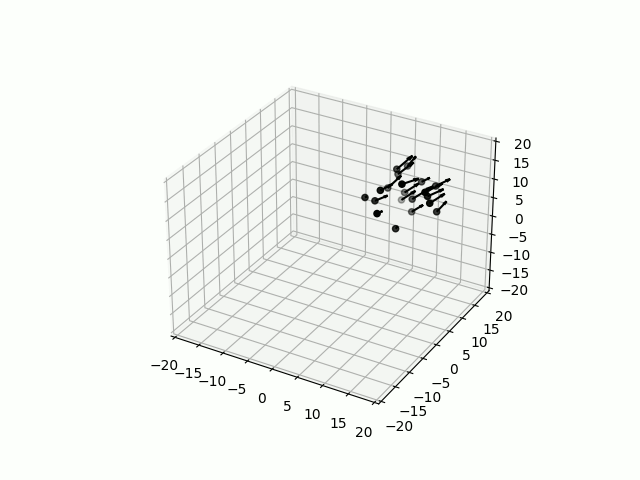
\includegraphics[width=0.7\linewidth]{images/page_garde.png}
	\vfill
	{\Large \@date}
	\rule{\linewidth}{0.4pt}
\end{titlepage}
\makeatother

\tableofcontents

\nnchapter{Introduction}


	Notre sujet est intitulé «~Modèle de \textsc{Vicsek}~». Le but de ce projet numérique est de reproduire de manière numérique le modèle de \textsc{Vicsek}.

	Le modèle de \textsc{Vicsek} a été crée par le scientifique Tamás \textsc{Vicsek}. Il s'agit d'un physicien hongrois connu pour ses contributions à la physique statistique, à la biologie et à la dynamique des systèmes. Il est né le 10 mai 1948 (~74 ans aujourd'hui~) à Budapest. Il est aujourd'hui professeur à l'Université Eötvös \textsc{Loránd} de Budapest. Ce brillant physicien est d'ailleurs un des membres de l'Académie hongroise des sciences et a reçu de nombreux prix pour ses contributions à la physique, notamment le prix \textsc{Széchenyi} (~en 1999~) ou encore le prix Lars \textsc{Onsager} (~en 2020~). \\

	Mais Tamás \textsc{Vicsek} est surtout connu pour son travail sur les systèmes auto-organisés~; ces modèles permettent d'étudier les mouvements collectifs. Il a ainsi travaillé sur le comportement d'agents individuels qui interagissent avec d'autres agents aux alentours, ses observations montrent que des motifs de mouvements collectifs emmergent d'eux-même.
	
	Le groupe se déplace alors de manière coordonnée sans qu'il n'y ait de leader comme on peut l'observer notamment dans la migration des grues. Nous pouvons citer comme exemples~: les bancs de poissons, les regroupements de certains oiseaux, les essaims d'insectes, ou encore le mouvement de foules.

	 Le premier modèle de \textsc{Vicsek} voit ainsi le jour en 1995.\\
	 
	
\chapter{Présentation et explications}	

	Le modèle de \textsc{Vicsek} permet d'étudier un groupe d'agents qui se déplace dans un espace.
	
	Chacun des agents a une vitesse donnée (~en norme et en direction~) et va interagir avec ses voisins. Ce qui concrètement se traduit par des changements concernant la norme et la direction de la vitesse.
	
	Nous nous attendons alors à observer la création d'un mouvement de groupe du aux interactions entre les agents. \\
	
	Cependant, les agents observables dans la vie réelle ne suivent pas toujours le groupe à la perfection, et il peut arriver qu'un agent s'écarte, de manière aléatoire, des autres. C'est pour cela que \textsc{Vicsek} a introduit une notion de bruit dans son modèle. En effet, à chaque pas de temps, chaque agent va prendre la direction moyenne des agents autour de lui et à cette direction va venir se superposer un bruit qui le fera peut-être dévier dans une autre direction.
	
	En augmentant significativement le bruit, le groupe pert son mouvement collectif et les agents prennent alors des directions aléatoires.\\

	Le modèle de \textsc{Vicsek} s'implémente très simplement puisqu'il se réduit à deux équations~:
	\[ \left\{ \begin{array}{rcl}
		\Theta_{i}(t + \text dt) & = & \Theta_{j |r_{i}-r_{j}|<r} + \eta_{i}(t) \\[0.2cm]
		r_{i}(t + \text dt) & = & r_{i}(t) + v_{i}\Delta t
	\end{array} \right. \]
	dans lesquelles $r_{i}$ la position de chaque individu donnée par un vecteur de position, nous prendrons $i$ comme indice de l'agent en question et $t$ le temps. Nous noterons également $\eta$ le bruit et $\Theta$ pour l’angle définissant la direction de sa vitesse. Ici, $\Theta_{j |r_{i}-r_{j}|<r}$ nous indiquera la direction moyenne des vitesses des agents dans un cercle de rayon $r$. L'indice $j$ repésentera alors l'ensemble des voisins de $i$ compris dans ce cercle.\\

	Ce qui est intéressant, c'est que nous pouvons, en modifiant certains paramètres du système étudié, observer un mouvement de foule plus fort ou plus faible. Nous pourrons alors jouer sur la surface et les dimensions du plan étudié, le nombre d'agent et donc par conséquent la densité de population et même le bruit.\\

	Le modèle de \textsc{Vicsek} est important pour étudier le comportement de certains animaux en biologie ou encore l'étude des foules. Ce modèle peut même être utile à la construction de bâtiment. En effet, le comportement des foules peut être intéressant dans la conception d'entrées et de sorties d'un espace fermé, notamment dans un moment de panique. La foule va s'éloigner du danger est emprunter les sorties. Il est alors crucial de prévoir le comportement des agents pour placer les sorties de manière à ce que le débit d'agent sortant soit le plus important possible.\\
	
	Nous pouvons également retrouver le modèle de \textsc{Vicsek} dans la robotique. C'est un précieux outil pour la technologie du monde moderne. Il peut être utiliser dans des programmes informatiques qui gèrent le déplacement de systèmes de robots (~comme les drones~).\\ 

	C'est avec tout cela que nous essayerons, à travers ce projet, de reproduire numériquement des mouvements collectifs et ainsi étudier le modèle de \textsc{Vicsek}.
	
\chapter{Méthode employée}
\section{Classes et méthodes}

    Pour ce projet, la programmation orientée objet s'est naturellement imposée. Nous utilisons ainsi deux classes principales appelées \verb|Agent| et \verb|Group| qui fixent respectivement les paramètres de l'agent et du groupe. Assez simplement, la classe \verb|Group| contient une liste d'instances de la classe \verb|Agent| et permet de les représenter dans l'espace et le temps. La classe \verb|Agent| permet d'encapsuler toutes les données de chaque agent~: position, vitesse et direction.
    
	Ainsi, nous pouvons retrouver dans chaque classe, plusieurs méthodes qui vont nous aider à mieux définir les groupes et les agents ainsi qu'à les faire évoluer. \\
   
\section{Début de la programmation}
	Nous avons commencé par programmer les classes avec des méthodes basiques qui permettaient d'initialiser, de faire évoluer et de représenter les agents.
   
	Une fois les deux équations implémentées, nous avons créé la fonction \verb|group_generator| qui nous permettait de créer simplement un groupe en prenant des paramètres aléatoires dans des limites fixées pour les agents.
   
	Après avoir créé notre groupe avec \verb|group_generator|, nous le faisions évoluer grâce à la méthode \verb|Group.run| et nous générions une image au format PNG en deux ou trois dimensions avec \verb|Group.compute_figure|. \\
	
	Cela nous a permis d'avoir des premières représentations de nos groupes d'agents~:
	\begin{figure}[!h]
		\centering
		\begin{tabular}{cc}
			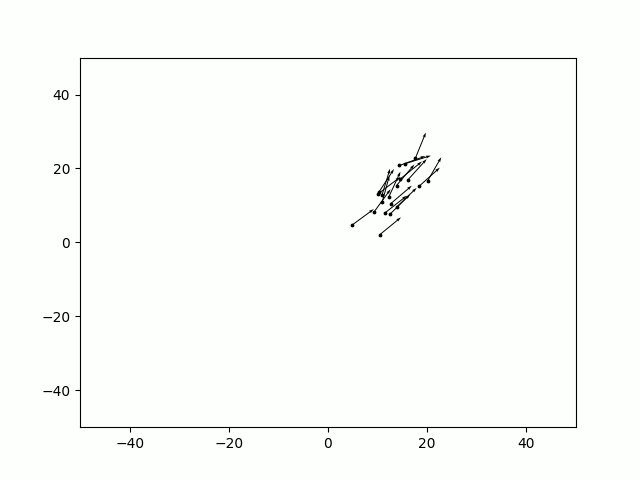
\includegraphics[width=8cm]{images/image_2.png} & 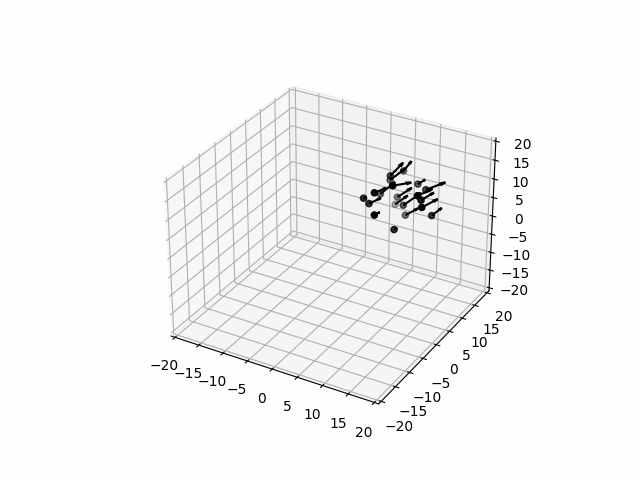
\includegraphics[width=10cm]{images/image_1.png} \\
		\end{tabular}
		\caption{Premières images obtenues en 2D et 3D }
	\end{figure} \newpage

\chapter{Premières interprétations physiques}
\section{Premiers résultats}

   Pour pouvoir observer un mouvement, il est plus utile de regarder une vidéo que des images. Nous avons alors créé une méthode~: \verb|Group.compute_animation| qui utilise la classe \verb|Artist_animation| du module \verb|matplotlib|. Nous arrivions alors à générer des fichiers GIF avec le nombre de frames souhaité.
   
   Après avoir généré plusieurs animations avec des groupes de tailles différentes. Nous avons pu déjà tirer quelques conclusions. En effet, nous observions des mouvements de groupes. Les agents qui avaient des positions de départ aléatoires, sont influencés les uns les autres selon la distance avec leurs voisins.
   
   On observe d'ailleurs des mouvements collectifs plus importants quand la densité d'agent est plus forte. En revanche, quand les agents sont moins nombreux dans un même espace, nous observons davantage de formations de petits groupes ou des agents solitaires. 
   
   Cela s'explique par le fait que les agents ne se voient plus.
   
	\begin{figure}[!h]
		\centering
		\begin{tabular}{cc}
			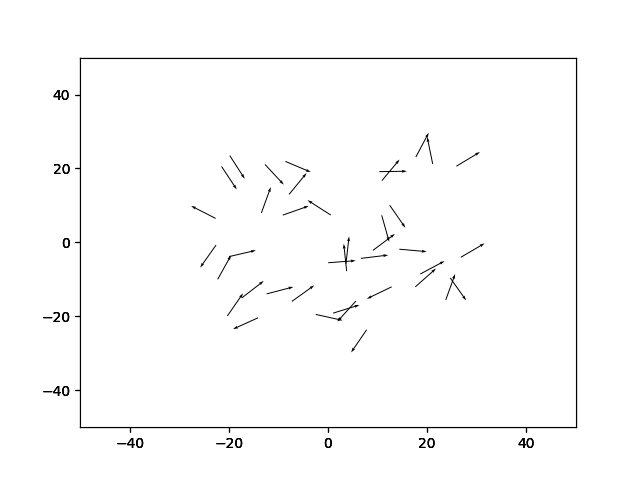
\includegraphics[width=8cm]{images/image_3.png} & 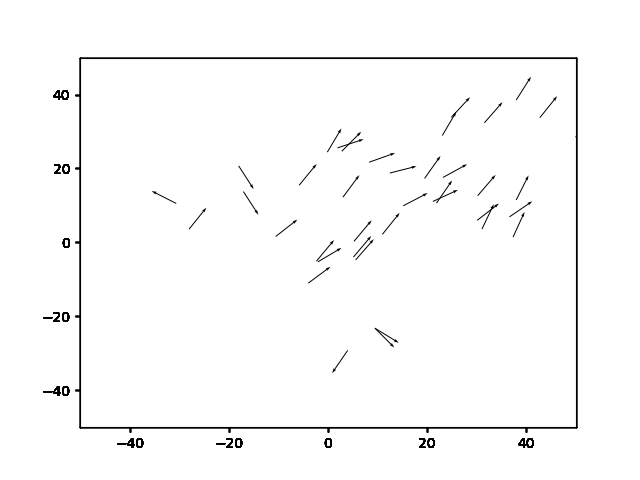
\includegraphics[width=8cm]{images/image_4.png} \\
		\end{tabular}
		\caption{Début et fin d'une animation 2D}
	\end{figure} 
   
   
\section{Mouvements de groupe}

   Pour mieux observer les mouvements de groupe, nous avons décidé de mettre une couleur à nos agents selon leur direction. Cela permet de mieux visuliser les différents groupe et de s'affranchir des flèches qui étaient devenue gênantes pour bien discerner le mouvement collectif à haute densité.
   
   Nous avons gardé cette représentation de l'angle des agents pour tout le reste du projet.
   
   \begin{figure}[!h]
		\centering
		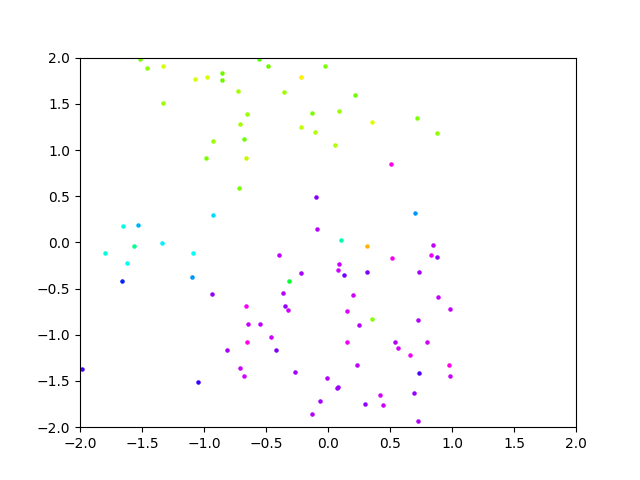
\includegraphics[width=10cm]{images/image_6.png}
		\caption{Image colorée pour la visualisation de groupe}
		\label{couleurs_image}
	\end{figure}  
   
   Sur cette nouvelle figure \ref{couleurs_image}, nous voyons bien les différents groupes crées. On distingue encore mieux les mouvements lors de l'animation.\\
   
   Nous avons d'ailleurs pu observer une organisation intéressante des agents sur certaines animations. En effet, les agents se regroupent premièrement en plusieurs petits groupes (~sur l'image de gauche de la figure \ref{mouvement_grp2}, on discerne en effet trois groupe principaux en violet, vert et cyan~). Enfin, les petits groupes s'unissent pour former un seul et même grand groupe.
   
    \begin{figure}[!h]
		\centering
		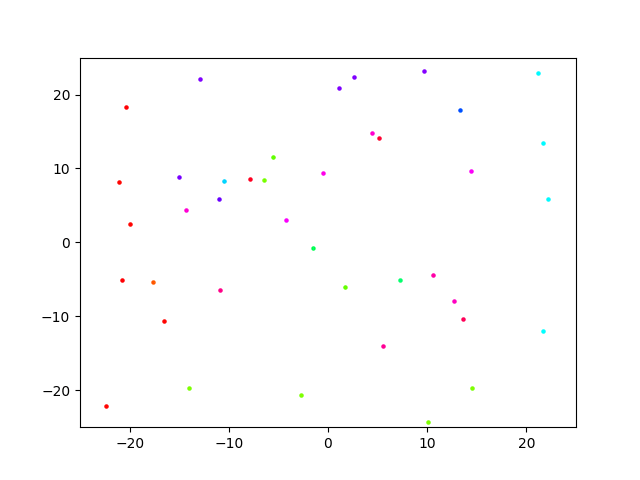
\includegraphics[width=10cm]{images/image_8.png}
		\caption{Image de départ }
		\label{mouvement_grp}
	\end{figure} 
	
   \begin{figure}[!h]
		\centering
		\begin{tabular}{cc}
			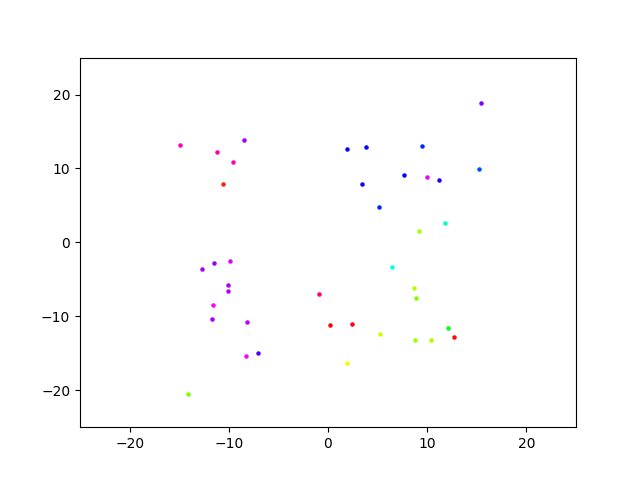
\includegraphics[width=8cm]{images/image_7.png} & 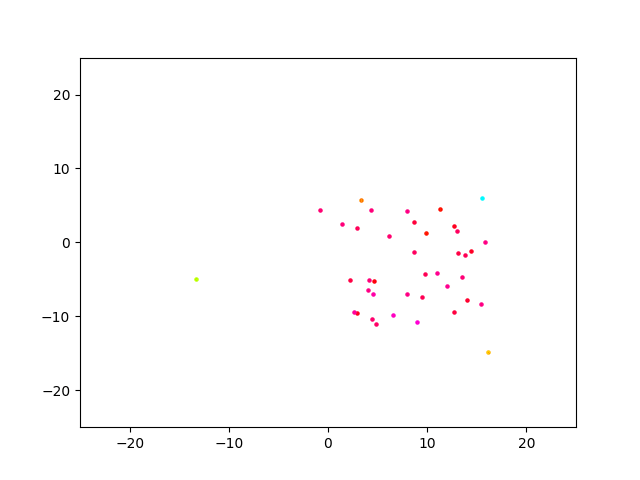
\includegraphics[width=8cm]{images/image_9.png} \\
		\end{tabular}
		\caption{Formations de petits groupe puis d'un seul et même groupe}
		\label{mouvement_grp2}
	\end{figure} 
	
	Ceci montre encore un fois très bien l'influence entre les agents.

\section{Paramètre de bruit}
    
   Nous avons déjà pu observer l'impact du bruit sur les populations. Nous voyons alors que ce paramètre est capital pour l'observation de mouvements collectifs. Si celui-ci est trop fort, les agents feront route seuls et ne s'occuperont pas du mouvement des voisins. En revanche, les mouvements collectifs seront davantages présents avec un bruit qui tend vers zéro.

Par exemple, en regardant ces images~:
   
	\begin{figure}[!h]
		\centering
		\begin{tabular}{cc}
			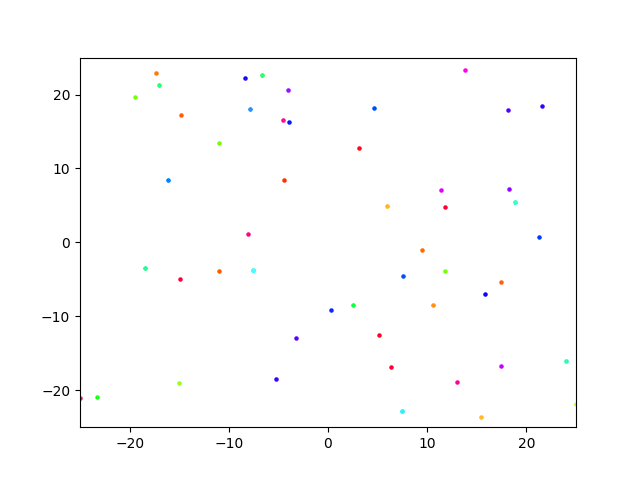
\includegraphics[width=8cm]{images/image_10.png} & 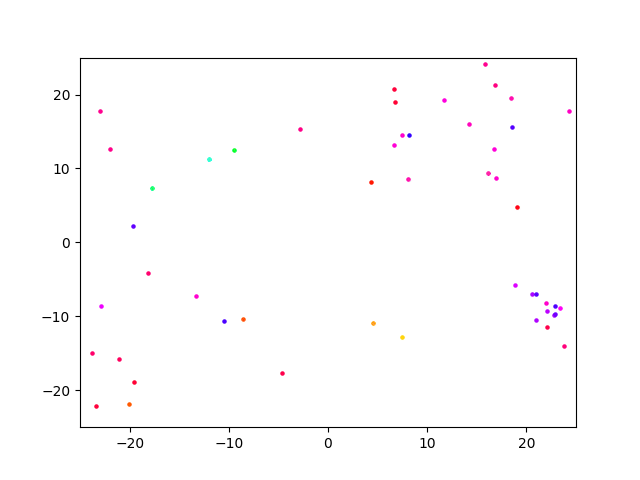
\includegraphics[width=8cm]{images/image_11.png} \\
		\end{tabular}
		\caption{Visualisation de l'impact du bruit (~début et fin d'animation~)}
	\end{figure} 
	
Nous voyons bien ici que les agents ont des directions plutôt différentes (~hormis un petit groupe de coordonnées (~25 ; -10~)~). Le bruit est fort dans ce cas, et les agents ont tendance à prendre des directions sans s'occuper de leurs voisins.
   
\chapter{Résultats expérimentaux}
\section{Résultats historiques de Viscek}
	Nous avons commencé par chercher à reproduire les résultats obtenus par Vicsek en reprenant les mêmes paramètres.
	
	Chaque agent n'est ainsi influencé que par ses plus proches voisins et évolue dans un espace torique. En laissant la densité constante et en faisant varier le bruit pour voir son influence sur le paramètre d'alignement, nous observons alors un profil de transition de phase.
	
	Sur la figure suivante chaque points est la moyenne sur cinq mesures de 200 pas et 50 agents.
	\begin{figure}[!h]
		\centering
		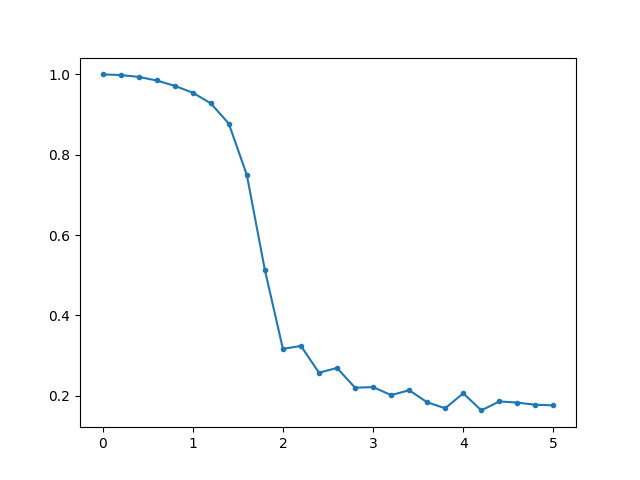
\includegraphics[width=12cm]{images/bruit_4.png}
		\caption{Paramètre d'alignement en fonction du bruit}
	\end{figure}
	
	Pour un bruit très faible, les agents sont alignés avec un paramètre d'alignement de 1 ce qui est cohérent puisqu'ils vont s'aligner sans aucune part d'aléatoire. Pour un bruit élevé, ce qui correspond en fait à une probabilité d'avoir une déviation angulaire importante par rapport à la direction moyenne, les agents sont très peu alignés pour un même nombre d'itération. \\
	
	Nous avons ici exactement les mêmes résultats que ceux obtenus par \textsc{Vicsek} et son équipe.

\section{Autres paramètres en jeu}
	\subsection{Cône de vision}
	
		Afin de mieux visualiser ce que peut voir un agent en particulier, nous avons alors décidé de rajouter un cône de vision.
		
		Nous serons ainsi capable de mieux voir comment un agent réagit selon ce qu'il voit. \\
		
		Ainsi, un agent un considéré comme voisin s'il est dans le cône de vision de l'agent testé. En refaisant le même test que précédemment, nous observons que les agents restent alignés moins longtemps.
		
		En effet, les agents étant plus sensible à l'orientation pour voir les autres, si le bruit augmente, les agents vont avoir des déviations angulaires plus importante et peuvent donc perdre de vue les autres agents plus facilement ce qui fait chuter le paramètre d'alignement plus rapidement.
	
	
   \begin{figure}[!h]
		\centering
		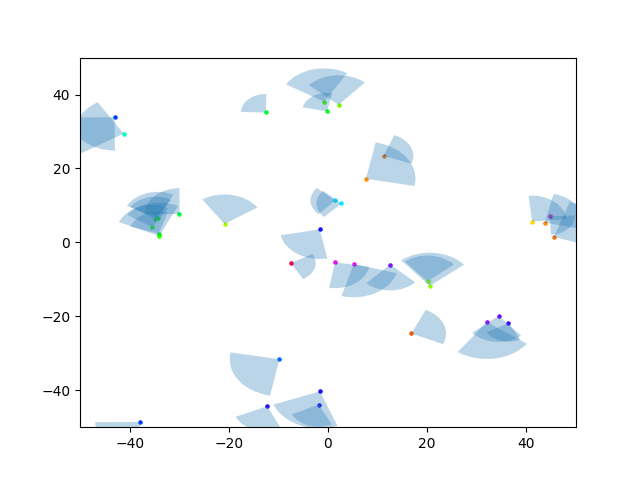
\includegraphics[width=10cm]{images/image_12.png}
		\caption{Image de l'animation générée avec cône de vision}
		\label{cone_vision}
	\end{figure}  
  
    Nous avons cependant préféré retirer ce cône dans la suite du projet. En effet, l'animation générée devenait trop chargée et riche en informations. Il était alors difficile de bien observer le comportement des agents.
    
    \subsection{Création d'un agent leader}
       
       Nous avons maintenant voulu nous écarté un peu du modèle de Viscek, en étudiant un nouveau type de mouvement collectif. Nous avons alors crée un nouveau type d'agent, dit leader, qui influence davantage les agents normaux. Nous pouvons définir à quel point celui-ci à de l'influence (~nous avons choisi une influence équivalente à 4 agents~).
       
       Nous nous attendions à observer des groupe en forme de pyramide. C'est à dire une organisation hiérarchique des agents pour créer un mouvement de groupe. Nous pouvons par exemple observer ce comportement chez certains animaux, notamment lors de la migrations des grues. 
       
       Nous avons choisi de représenter l'agent leader en noir.
       
       [IMAGES]
    
       
       Nous avons d'ailleurs pu observer quelque chose d'intéressant. En effet, sur une animation, nous pouvons voir un groupe d'agent qui suit l'agent leader pendant un moment. Mais, ce groupe croise un autre groupe d'agent. Les agents qui suivait l'agent leader se sont mis subitement à suivre le nouveau groupe. 
       
       \begin{figure}[!h]
		\centering
		\begin{tabular}{cc}
			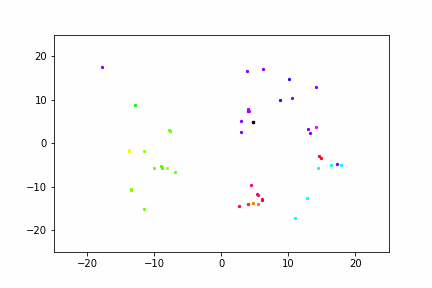
\includegraphics[width=8cm]{images/image_13.png} & 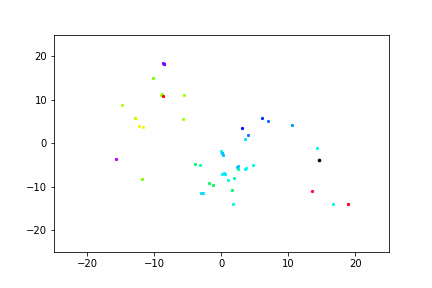
\includegraphics[width=8cm]{images/image_14.png} \\
		\end{tabular}
		\caption{Situation intéressante avec un agent leader}
	\end{figure}
       
       Ainsi, nous en déduisons que le groupe a eu plus d'influence que l'agent leader à ce moment là.
       
       
   \subsection{Mise en place d'une prédation}
       
       Nous avons trouvé intéressant de rajouter des agents dit répulsifs, qui joue le rôle de prédateurs. Ces nouveaux agents sont plus rapides que leurs proies. Ainsi, nous avons pu voir comment s'organisent les agents face à la menace. 
       
       [IMAGES AVEC AGENT SEUL AU MILIEU ECT]
       
       
   

	\subsection{Système évolutif}
	
		En ajoutant les agents répulsifs, nous avons eu l'idée de créer un système de «mort» où les agents touchés par un agent répulsifs sont retirés de la liste des agents et placés dans un autre attribut du groupe. Cela permet notamment de comparer les caractéristiques des agents morts avec celles des survivants et de voir quels paramètres permettent de survivre. En mettant des valeurs limites pour le bruit et la sensibilité aux agents répulsifs et en moyennant les résultats sur 10 mesures, nous obtenons les résultats suivants~:
		
		\begin{tabular}{|c|c|c|} \hline
			bruit & sensibilité & pourcentage de survivants \\ \hline
			1 & 0 & 30 \\ \hline
			0 & 1 & 79 \\ \hline
			1 & 1 & 86 \\ \hline
			0 & 0 & 39 \\ \hline
		\end{tabular}

\subsection{Ajout d'obstacles}
	
\end{document}
